\documentclass{sig-alternate}
\usepackage{multirow}
\usepackage{multicol}
\usepackage{listings}
\usepackage{color}
\usepackage[anythingbreaks]{breakurl}
\begin{document}
\conferenceinfo{CSC766}{'15 Spring Raleigh, North Carolina USA}

\title{Ontology-based Knowledge Representation for PORPLE}
\subtitle{[CSC766 Final Report]}

\numberofauthors{3}
\author{
\alignauthor
Feifei Wang\\
       \affaddr{North Carolina State University}\\
       \email{fwang12@ncsu.edu}
\alignauthor
Yue Zhao\\
       \affaddr{North Carolina State University}\\
       \email{yzhao30@ncsu.edu}
\alignauthor
Xipeng Shen\\
       \affaddr{North Carolina State University}\\
       \email{xshen5@ncsu.edu}
}
\maketitle
\begin{abstract}
Data placement is important for the performance of a GPU (Graphic Processing Unit) program. However, where to place the data is a complex decision for a programmer to make. Among the recent techniques in solving data placement problem, PORPLE is a representative one. PORPLE is a portable data placement engine that uses hardware information (memory systems and processors) described by memory specification language (MSL) and software information (data access patterns) gathered from a compiler called PORPLE-C. Because of the two different representations, it is hard to share common understanding of the program, and reuse information. Providing a more general, uniform and reusable representation can make data replacement decisions more efficient, interoperable and reusable.

In this paper, we apply ontology-based techniques to systematically and formally represent both hardware information and software information used by PORPLE hoping to achieve efficiency, interoperability and reusability. Specifically, we transform the information of GPU memory systems and processors, and the data access patterns gathered by PROPLE-C to ontology, which can be used by PORPLE for data replacement.
 
\end{abstract}

\terms{Compiler}

\keywords{compiler, ontology, data placement}

\section{Introduction}
Data placement is essential for the performance of a GPU (Graphic Processing Unit) program \cite{related1}. However, where to place the data depends on the hardware information of the GPU and software information of the program and its input. The hardware information of the GPU includes its memory systems and processors, while the software information means the data access patterns associated with the input to the programs. The memory systems of GPUs are becoming increasingly complex. For example, there exists more than eight types of memory (including caches) on the Tesla M2075 GPU. These memories have different size limitations, block sizes, access constraints and \texttt{etc.} Also, the suitable placements depends on the program inputs since different inputs to a program may lead to different data access patterns, and thus require different data placement. As a result, data placement problem is difficult but should be solved.

There have been some efforts to address the data placement problem \cite{related1, related2, related3, porple}. Among them, PORPLE \cite{porple} is a representative one because it considers various types of GPU programs. PORPLE is a portable data placement engine that takes both hardware information (memory systems and processors) and software information (data access patterns) into consideration and uses them to make data placement decisions. PORPLE obtains information about memory systems and processors from memory specification language (MSL), and uses the runtime profiling to acquire the data access patterns. In such a sense, PORPLE uses two different types of representations, which makes it hard to share common understanding of the program and reuse information. Providing a more general, uniform and reusable representation can improve the efficiency, interoperability and reusability of PORPLE and potentially some other work.

There exists various techniques to represent knowledge \cite{intro2}. Recently, ontology-based knowledge bases are becoming increasingly popular. Ontology is a general-purpose modeling for knowledge resources. It is used to define a common vocabulary and a shared understanding explicitly \cite{ontology1, ontology2}. It has been successfully used to build knowledge bases in many fields \cite{ontology3, ontology4, ontology5, ontology6, work1, work2}. Motivated by their advances, we choose ontology as the representation.

In this paper, we apply ontology-based techniques to systematically and formally represent both hardware information and software information hoping to make PORPLE more efficient, interoperable and reusable. Specifically, we transform the information of GPU memory systems and processors, and the data access patterns gathered to ontology, which can be used by PORPLE for data replacement. Note that although our work is designed for PORPLE, it can also be applied to other work.

This paper is organized as follows. In Section 2, we present the motivation of our work. Section 3 illustrates the challenges of the project, our solutions, and lessons we learned. In Section 4 we explain our implementation in detail. Section 5 shows the results. Section 6 concludes the paper and discusses some possible future work.

\section{Motivation}
This work is mainly motivated by an observation that PORPLE uses two different representations for hardware information and software information. Hardware information is represented by memory specification language (MSL), which is a carefully designed small specification language. It describes the memory systems of a GPU. Figure \ref{fig:msl} shows the MSL specification of the \texttt{Tesla M2075} GPU as an example. The MSL describes the properties of a type of memory and its relations with other pieces of memory in a system. For example, the second line of the file shows the properties of \texttt{globalMem}. The \textit{name} of the memory is \texttt{globalMem}, its \textit{id} is \texttt{8}, it is \textit{software manageable}, allows \texttt{read} and \texttt{write} accesses, and \texttt{etc.} It also shows the relations between \texttt{globalMem} and \texttt{L2} is that \texttt{globalMem} has an \textit{upper level} called \texttt{L2}. Software information, which is data access patterns, is represented by a form defined by \texttt{Chen et al.} \cite{porple} Figure \ref{fig:dap} presents one data access pattern used by PORPLE. In this file, the second line shows that the \textit{total memory access time} is \texttt{64}, \textit{L1 cache hit} is \texttt{0}, and \textit{L2 cache hit} is \texttt{0}.

Due to the two different representations, it is hard for them to share common understanding of the program and reuse information. In such a sense, we are motivated to choose ontology as a more general, uniform and reusable representation hoping to improve the efficiency, interoperability and reusability of PORPLE and potentially some other work.

This work is also motivated by the success of some previous work of using ontology to systematically represent, reuse, and manipulate software information, hardware information and optimization information. For example, OpenK adapts ontology-based techniques to build open and reusable knowledge bases to do program analysis and optimization in HPC. \texttt{Sosnovsky et al.} \cite{work1} and \texttt{Ganapathi et al.} \cite{work2} use ontology to teach abstract programming language. \texttt{Moor et al.} \cite{ontology3} and \texttt{Leenheer et al.} \cite{ontology4} focus on community-based evolution of knowledge-intensive systems with ontology. \texttt{Tang et al.} \cite{ontology5} implement a profile compiler that support ontology-based, community-grounded, multilingual, collaborative group decision making by leveraging ontology. 

\begin{figure*}
\centering
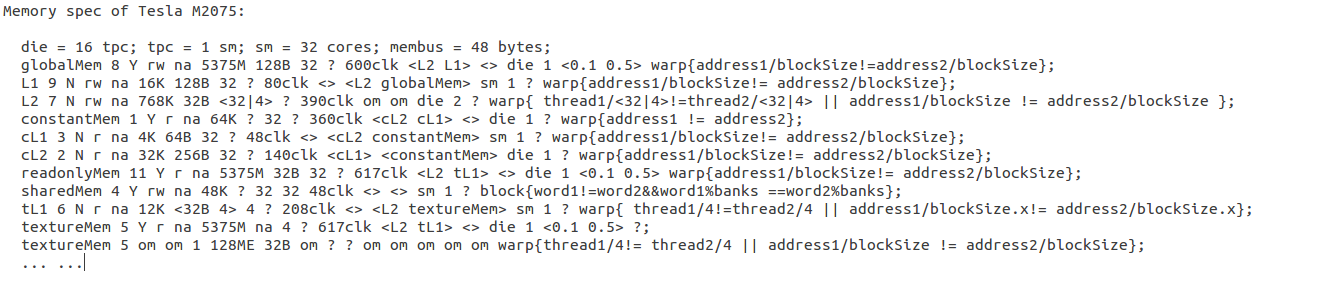
\epsfig{file=msl.png,height=4cm}
\caption{The memory specification of Tesla M2075 in MSL}
\label{fig:msl}
\end{figure*}

\begin{figure}
\centering
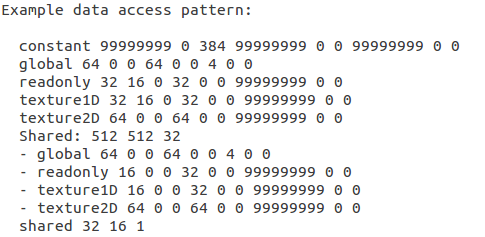
\epsfig{file=dap.png,height=4cm}
\caption{The data access pattern used by PORPLE}
\label{fig:dap}
\end{figure}

\begin{figure*}
\centering
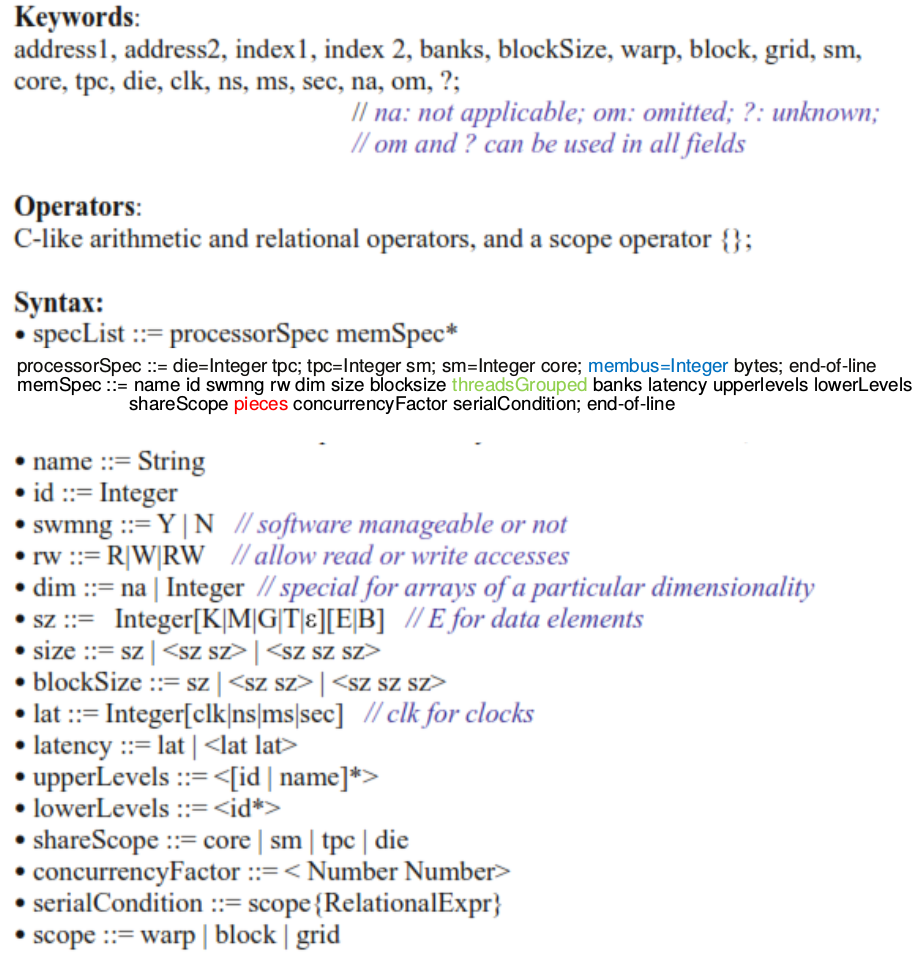
\epsfig{file=property.png,height=10cm}
\caption{Syntax of MSL}
\label{fig:property}
\end{figure*}

\section{Challenges, Solutions and Lessons}
Transforming MSL and data access patterns used by PORPLE to ontolgoy is quite straightforward. We have not met many challenges. The main challenge is to understand ontology. In this section, we introduce the challenges we met to understand ontology, how we overcame them, and the lessons we learned.

\subsection{Challenges}
Ontologies have three parts: individuals, properties and classes \cite{what1}. Individuals are objects in the domain in which we are interested. Properties represent binary relations between two individuals. Objects with similar characteristics are grouped by classes. In this part we use Figure \ref{fig:msl} as an example to illustrate the challenges we had to understand ontology. 

For the individual part, there are mainly two challenges. The first challenge is to use unique \texttt{namedIndividual} for each type of memory system. For example, in the MSL for \texttt{Tesla M2075}, although there are four \texttt{textureMem} with the same name, we cannot use the same name \texttt{textureMem} for all of them. We need to make sure that every \texttt{namedIndividual} is unique. The second challenge is that we cannot only create the memory types as \texttt{namedIndividual}, e.g. \texttt{L1} and \texttt{L2}. We must also consider the GPU vendors and types, e.g., \texttt{M2075}, \texttt{M2075GlobalMemory} and \texttt{M2075ConstantMemory}.

The challenge in understanding the property is that we need to consider \textit{inverse property}. Inverse property means that if a property links individual A to individual B then its inverse property should also link individual B to individual A \cite{what1}. For example, if \texttt{globalMem} has an upper level that is \texttt{L2}, then \texttt{L2} should have a lower level that is \texttt{globalMem}. 

For the class part, the challenge is to consider some characteristics that are not so obvious. For example, \texttt{L1} is a sub-class of \texttt{Cache} is obvious. However, we need to pay attention that \texttt{M2075} is a sub-class of \texttt{Tesla}, \texttt{M2075Processor} is a sub-class of \texttt{Processor}, \texttt{M2075GlobalMemory} is a sub-class of \texttt{GlobalMemory} and \texttt{etc.}

\subsection{Solutions}
Our solution is to use Prot{\'e}g{\'e} \cite{protege} to generate ontology files, and then learn from those generated files. By learning from Prot{\'e}g{\'e}, we learn to define individuals and arrange them into a hierarchy (sub-class hierarchy). We take \texttt{Tesla}, \texttt{M2075}, \texttt{Processor}, \texttt{scope}, \texttt{GlobalMemory}, \texttt{ConstantMemory}, \texttt{TextureMemory}, \texttt{Cache} and \texttt{etc.} into consideration. We also learn to define the properties that should be assigned to each class and give them values.

\subsection{Lessons}
The lessons we learned are that when creating ontology, we must think comprehensively. For example, we cannot just use the memory types as \texttt{namedIndividual}, e.g. \texttt{L1} and \texttt{L2}. We must also consider the GPU vendors and types, e.g., \texttt{M2075}, \texttt{M2075GlobalMemory} and \texttt{M2075ConstantMemory}. Similarly, when constructing the sub-class hierarchy, we cannot only consider the obvious ones such as \texttt{L1} is a sub-class of \texttt{Cache}. We must also consider that \texttt{M2075} is a sub-class of \texttt{Tesla}, and \texttt{M2075GlobalMemory} is also a sub-class of \texttt{GlobalMemory}. Also when assigning properties to \texttt{namedIndividual}, we have to think carefully about whether these properties have some special attributes such as inverse property. For example, if we give \texttt{globalMem} an upper level that is \texttt{L2}, then we should also give \texttt{L2} a lower level that is \texttt{globalMem}. 

\section{Implementation}
We have designed two implementations for MSL and data access patterns. We first introduce the implementation for MSL in detail, and then describe the implementation for data access patterns.

\subsection{MSL}
When transforming MSL to ontology, we first create individuals, then enumerate properties about them, and assert class descriptions about them in the end.

To create individuals, we first need to add various types of memory systems to our ontology. For example, \texttt{globalMem}, \texttt{constantMem}, \texttt{sharedMem}, are regarded as individuals. Note that when we add them, we must make sure that these memory systems is associated with \texttt{M2075}. As a result, we make them new names by adding \texttt{M2075} as a prefix and make the names become \texttt{M2075GlobalMemory}, \texttt{M2075ConstantMemory}, \texttt{M2075SharedMemory} and \texttt{etc.} We create \texttt{namedIndividual} for each of the memory systems since they are given an explicit name that can be used in any ontology to refer to the same object. After that, we must also add keywords such as \texttt{block}, \texttt{core}, \texttt{wrap} as namedIndividual.

After that, we enumerate the properties of individuals. We consider the properties as shown by Figure \ref{fig:property}, which is used by PORPLE \cite{porple}. By parsing the input file, we can get the information we need to create properties. We use two kinds of properties:

\begin{itemize}
	\item \texttt{ObjectPropertyAssertion}. ObjectPropertyAssertion allows one to state that an individual is connected by an object property expression to an individual. In MSL, we can get information about ObjectPropertyAssertion such as \texttt{hasBlockSize}, \texttt{hasLatency}, \texttt{hasLowerLevel} and \texttt{etc.}
	\item \texttt{DataPropertyAssertion}. DataPropertyAssertion allows one to state that an individual is connected by a data property expression to a literal. In MSL, we can get information about DataPropertyAssertion such as \texttt{CoresPerSM}, \texttt{numberofCoresValue}, \texttt{threadsPerBlock} and \texttt{etc.}
\end{itemize}

In the end, we define sub-class hierarchy to state that an individual is an instance of a particular class. For example, \texttt{M2075ConstantMemory} is a sub-class of \texttt{ConstantMemory}, \texttt{M2075GlobalMemory} is a sub-class of \texttt{GlobalMemory}, \texttt{cL1} is a sub-class of \texttt{L1\_constant} and \texttt{etc.} 

\subsection{Data Access Patterns}
Transforming data access patterns to ontology is quite easy since the syntax and semantics of data access patterns is simple. For example, Figure \ref{fig:dap} shows an example input file. For this input file, we only need to create \texttt{namedIndividual} for the memory types. For properties, we group the numbers following the names into groups of three numbers as designed by \texttt{Chen et al.} \cite{porple} We only need to consider four properties here:

\begin{itemize}
	\item \textit{Total memory access time}. Total memory access time is the first number in the group.
	\item \textit{L1 cache hit}. L1 cache hit is the second number in the group.
	\item \textit{L2 cache hit}. L2 cache hit is the third number in the group.
	\item \textit{Off-chip memory access time}. Off-chip memory access time is total memory access time minus L1 cache hit and minus L2 cache hit.
\end{itemize}

Note that when parsing the input file, we neglect numbers begin with \texttt{9} since they are considered not applicable by PORPLE \cite{porple}.

Also, for data access patterns, they do not have the sub-class hierarchy. 

\section{Results}

\begin{figure*}
\centering
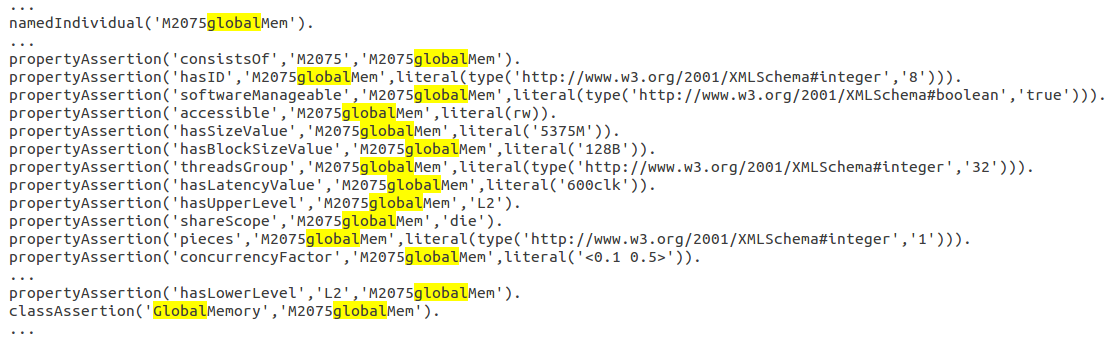
\epsfig{file=output1.png,height=6.5cm}
\caption{Example ontology representation for MSL}
\label{fig:output1}
\end{figure*}

\begin{figure*}
\centering
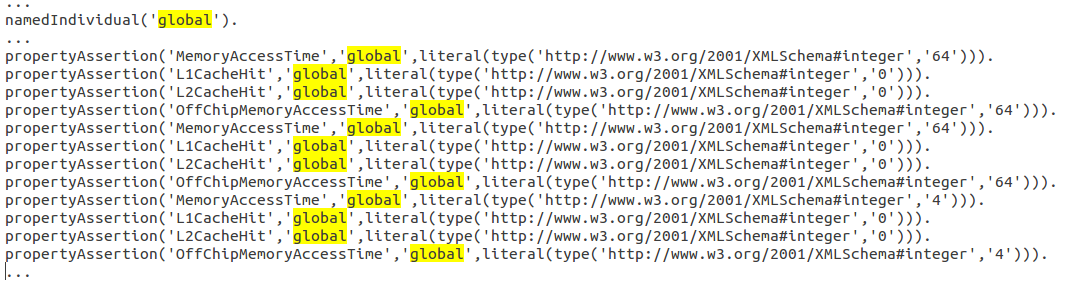
\epsfig{file=output2.png,height=5cm}
\caption{Example ontology representation for data access patterns}
\label{fig:output2}
\end{figure*}

Figure \ref{fig:output1} shows the results of transforming MSL to ontology, and Figure \ref{fig:output2} shows the results of transforming data access patterns to ontology. In this section, we first explain Figure \ref{fig:output1}, and then explain Figure \ref{fig:output2}.

\subsection{Ontology representation for MSL}

In Figure \ref{fig:output1}, the output result consists of three parts:
\begin{itemize}
	\item namedIndividual. 
	\item propertyAssertion. 
	\item classAssertion. 
\end{itemize}

For example, \texttt{namedIndividual('M2075globalMem')} means that \texttt{M2075globalMem} is a particular kind of memory system. It can be used in \texttt{propertyAssertion} and \texttt{classAssertion}.

There are a lot of \texttt{propertyAssertion}. We list a few properties here as some examples of how to illustrate the ouput.

\begin{itemize}
	\item \texttt{propertyAssertion('consistsOf', 'M2075', 'M2075globalMem')} means that \texttt{M2075globalMem} is consisted of by \texttt{M2075}.
	\item \texttt{propertyAssertion('hasID', 'M2075globalMem', literal(type('http://www.w3.org/2001/XMLSchema\#integer', '8')))} means that \texttt{M2075globalMem} has an ID which is \texttt{8}.
	\item \texttt{propertyAssertion('softwareManageable', 'M2075globalMem', literal(type('http://www.w3.org/2001/XMLSchema\#boolean', 'true')))} means that \texttt{M2075globalMem} is software manageable.
	\item \texttt{propertyAssertion('accessible', 'M2075globalMem', literal(rw))} means that \texttt{M2075globalMem} has read and write access.
	\item \texttt{propertyAssertion('hasSizeValue', 'M2075globalMem', literal('5375M'))} has a size of \texttt{128B}.
	\item \texttt{propertyAssertion('hasBlockSizeValue', 'M2075globalMem', literal('128B'))} means that the block size of \texttt{M2075globalMem} is \texttt{128B}.
	\item \texttt{propertyAssertion('threadsGroup', 'M2075globalMem', literal(type('http://www.w3.org/2001/XMLSchema\#integer', '32')))} means that \texttt{M2075globalMem} has threadGroup of \texttt{32}.
	\item \texttt{propertyAssertion('hasLatencyValue', 'M2075globalMem', literal('600clk'))} means the latency value of \texttt{M2075globalMem} is \texttt{600clk}.
	\item \texttt{propertyAssertion('hasUpperLevel', 'M2075globalMem', 'L2')} means that \texttt{M2075globalMem} has an upper level that is \texttt{L2}.
\end{itemize}

Since \texttt{M2075globalMem} is a kind of GlobalMemory, we need to construct a sub-class hierarchy that by specifying \texttt{classAssertion('GlobalMemory','M2075globalMem')}.

\subsection{Ontology representation for Data Access Patterns}

In Figure \ref{fig:output2}, there are only two parts:
\begin{itemize}
	\item namedIndividual. 
	\item propertyAssertion. 
\end{itemize}

For example, \texttt{namedIndividual('global')} means that this access pattern is for global memory system. It is also used in \texttt{propertyAssertion} and \texttt{classAssertion}.

There are only four kinds of properties for data access patterns.

\begin{itemize}
	\item \texttt{propertyAssertion('MemoryAccessTime', 'global', literal(type('http://www.w3.org/2001/XMLSchema\# integer', '64')))} means that global memory access time is \texttt{64}.
	\item \texttt{propertyAssertion('L1CacheHit', 'global', literal (type('http://www.w3.org/2001/XMLSchema\#integer', '0')))} means that L1 cache hit is \texttt{0}.
	\item \texttt{propertyAssertion('L2CacheHit', 'global', literal (type('http://www.w3.org/2001/XMLSchema\#integer', '0')))} means that L2 cache hit is \texttt{0} too.
	\item \texttt{propertyAssertion('OffChipMemoryAccessTime','global ', literal(type('http://www.w3.org/2001/XMLSchema\# integer', '64')))} means that the off-chip memory access time is \texttt{64}.
\end{itemize}

\section{Conclusion and Future Work}
Data placement has a great influence on GPU programs, which makes data placement problem an important issue for GPU program performance. Current techniques to solve data placement problem use different representations of information, e.g., PORPLE, which is hard to share common understanding of the program, and reuse information. 

We provide a more general, uniform and reusable representation by using ontology-based techniques to make data replacement decisions more efficient, interoperable and reusable. In our work, we transform the information of GPU memory systems and processors, and the data access patterns gathered by PROPLE-C to ontology which can be used by PORPLE for data replacement.

Although our work is designed for PORPLE, it can be applied to other work as well. In the future, we may want to transform more memory related representatiions to ontology to achieve a more general information sharing and reuse.

\section{Acknowledgments}
Dr. Xipeng Shen helped me to choose the topic for the final project of CSC766. Yue Zhao and Guoyang Chen offered me a lot of help to get start with this project. The OpenK project developed by Chunhua Liao et al. helped enhance the presentation of the project.

\bibliographystyle{abbrv}
\bibliography{sigproc} 

\end{document}
\begin{thebibliography}{10}

\bibitem{porple}
G.~Chen, B.~Wu, D.~Li, and X.~Shen.
\newblock Porple: An extensible optimizer for portable data placement on gpu.
\newblock In {\em Microarchitecture (MICRO), 2014 47th Annual IEEE/ACM
  International Symposium on}, pages 88--100. IEEE, 2014.

\bibitem{ontology4}
P.~De~Leenheer and R.~Meersman.
\newblock Towards community-based evolution of knowledge-intensive systems.
\newblock In {\em On the Move to Meaningful Internet Systems 2007: CoopIS, DOA,
  ODBASE, GADA, and IS}, pages 989--1006. Springer, 2007.

\bibitem{ontology3}
A.~De~Moor, P.~De~Leenheer, and R.~Meersman.
\newblock Dogma-mess: A meaning evolution support system for
  interorganizational ontology engineering.
\newblock In {\em Conceptual structures: Inspiration and application}, pages
  189--202. Springer, 2006.

\bibitem{work2}
G.~Ganapathi, R.~Lourdusamy, and V.~Rajaram.
\newblock Towards ontology development for teaching programming language.
\newblock In {\em World Congress on Engineering}, 2011.

\bibitem{protege}
J.~H. Gennari, M.~A. Musen, R.~W. Fergerson, W.~E. Grosso, M.~Crub{\'e}zy,
  H.~Eriksson, N.~F. Noy, and S.~W. Tu.
\newblock The evolution of prot{\'e}g{\'e}: an environment for knowledge-based
  systems development.
\newblock {\em International Journal of Human-computer studies}, 58(1):89--123,
  2003.

\bibitem{ontology1}
T.~R. Gruber.
\newblock Toward principles for the design of ontologies used for knowledge
  sharing?
\newblock {\em International journal of human-computer studies},
  43(5):907--928, 1995.

\bibitem{ontology2}
N.~Guarino.
\newblock Formal ontology, conceptual analysis and knowledge representation.
\newblock {\em International journal of human-computer studies},
  43(5):625--640, 1995.

\bibitem{what1}
M.~Horridge, H.~Knublauch, A.~Rector, R.~Stevens, and C.~Wroe.
\newblock A practical guide to building owl ontologies using the
  prot{\'e}g{\'e}-owl plugin and co-ode tools edition 1.0.
\newblock {\em University of Manchester}, 2004.

\bibitem{related1}
B.~Jang, D.~Schaa, P.~Mistry, and D.~Kaeli.
\newblock Exploiting memory access patterns to improve memory performance in
  data-parallel architectures.
\newblock {\em Parallel and Distributed Systems, IEEE Transactions on},
  22(1):105--118, 2011.

\bibitem{ontology6}
A.~S. Kleshchev.
\newblock How can ontologies contribute to software development?
\newblock In {\em Knowledge Processing and Data Analysis}, pages 121--135.
  Springer, 2011.

\bibitem{related2}
W.~Ma and G.~Agrawal.
\newblock An integer programming framework for optimizing shared memory use on
  gpus.
\newblock In {\em High Performance Computing (HiPC), 2010 International
  Conference on}, pages 1--10. IEEE, 2010.

\bibitem{work1}
S.~Sosnovsky and T.~Gavrilova.
\newblock Development of educational ontology for c-programming.
\newblock 2006.

\bibitem{ontology5}
Y.~Tang, S.~Christiaens, K.~Kerremans, and R.~Meersman.
\newblock Profile compiler: Ontology-based, community-grounded, multilingual
  online services to support collaborative decision making.
\newblock In {\em Research Challenges in Information Science, 2008. RCIS 2008.
  Second International Conference on}, pages 279--288. IEEE, 2008.

\bibitem{intro2}
F.~Van~Harmelen, V.~Lifschitz, and B.~Porter.
\newblock {\em Handbook of knowledge representation}, volume~1.
\newblock Elsevier, 2008.

\bibitem{related3}
B.~Wang, B.~Wu, D.~Li, X.~Shen, W.~Yu, Y.~Jiao, and J.~S. Vetter.
\newblock Exploring hybrid memory for gpu energy efficiency through
  software-hardware co-design.
\newblock In {\em Proceedings of the 22nd international conference on Parallel
  architectures and compilation techniques}, pages 93--102. IEEE Press, 2013.
\end{thebibliography}
